%\documentclass[dvipdfmx]{beamer}      % platex の場合
\documentclass[handout]{beamer}         % lualatex の場合
\usepackage{mySld}

\begin{document}
\title{基礎コンピュータ工学\\第4章 マイコンの構成と操作}
\date{}

\begin{frame}
  \titlepage
  \centerline{\url{https://github.com/tctsigemura/TecTextBook}}
  \vfill
  \centerline{本スライドの入手:
    \raisebox{-7mm}{\includegraphics[scale=0.3]{../Img/QRs4.png}}}
\end{frame}

%==============================================================================
%\begin{frame}
%  \frametitle
%  \tableofcontents
%\end{frame}

\section{マイコンの操作}
%==============================================================================
\begin{frame}
  \frametitle{各部の名称}
  \vfill
  \centerline{
    \includegraphics[width=0.95\textwidth]{../Keynote/kakubu-crop.pdf}}
  \vfill
  \begin{itemize}
    \item ビデオ(各部の名称,前半)
  \end{itemize}
  \vfill
\end{frame}

%==============================================================================
\begin{frame}
  \frametitle{コンソールパネル}
  \vfill
  \centerline{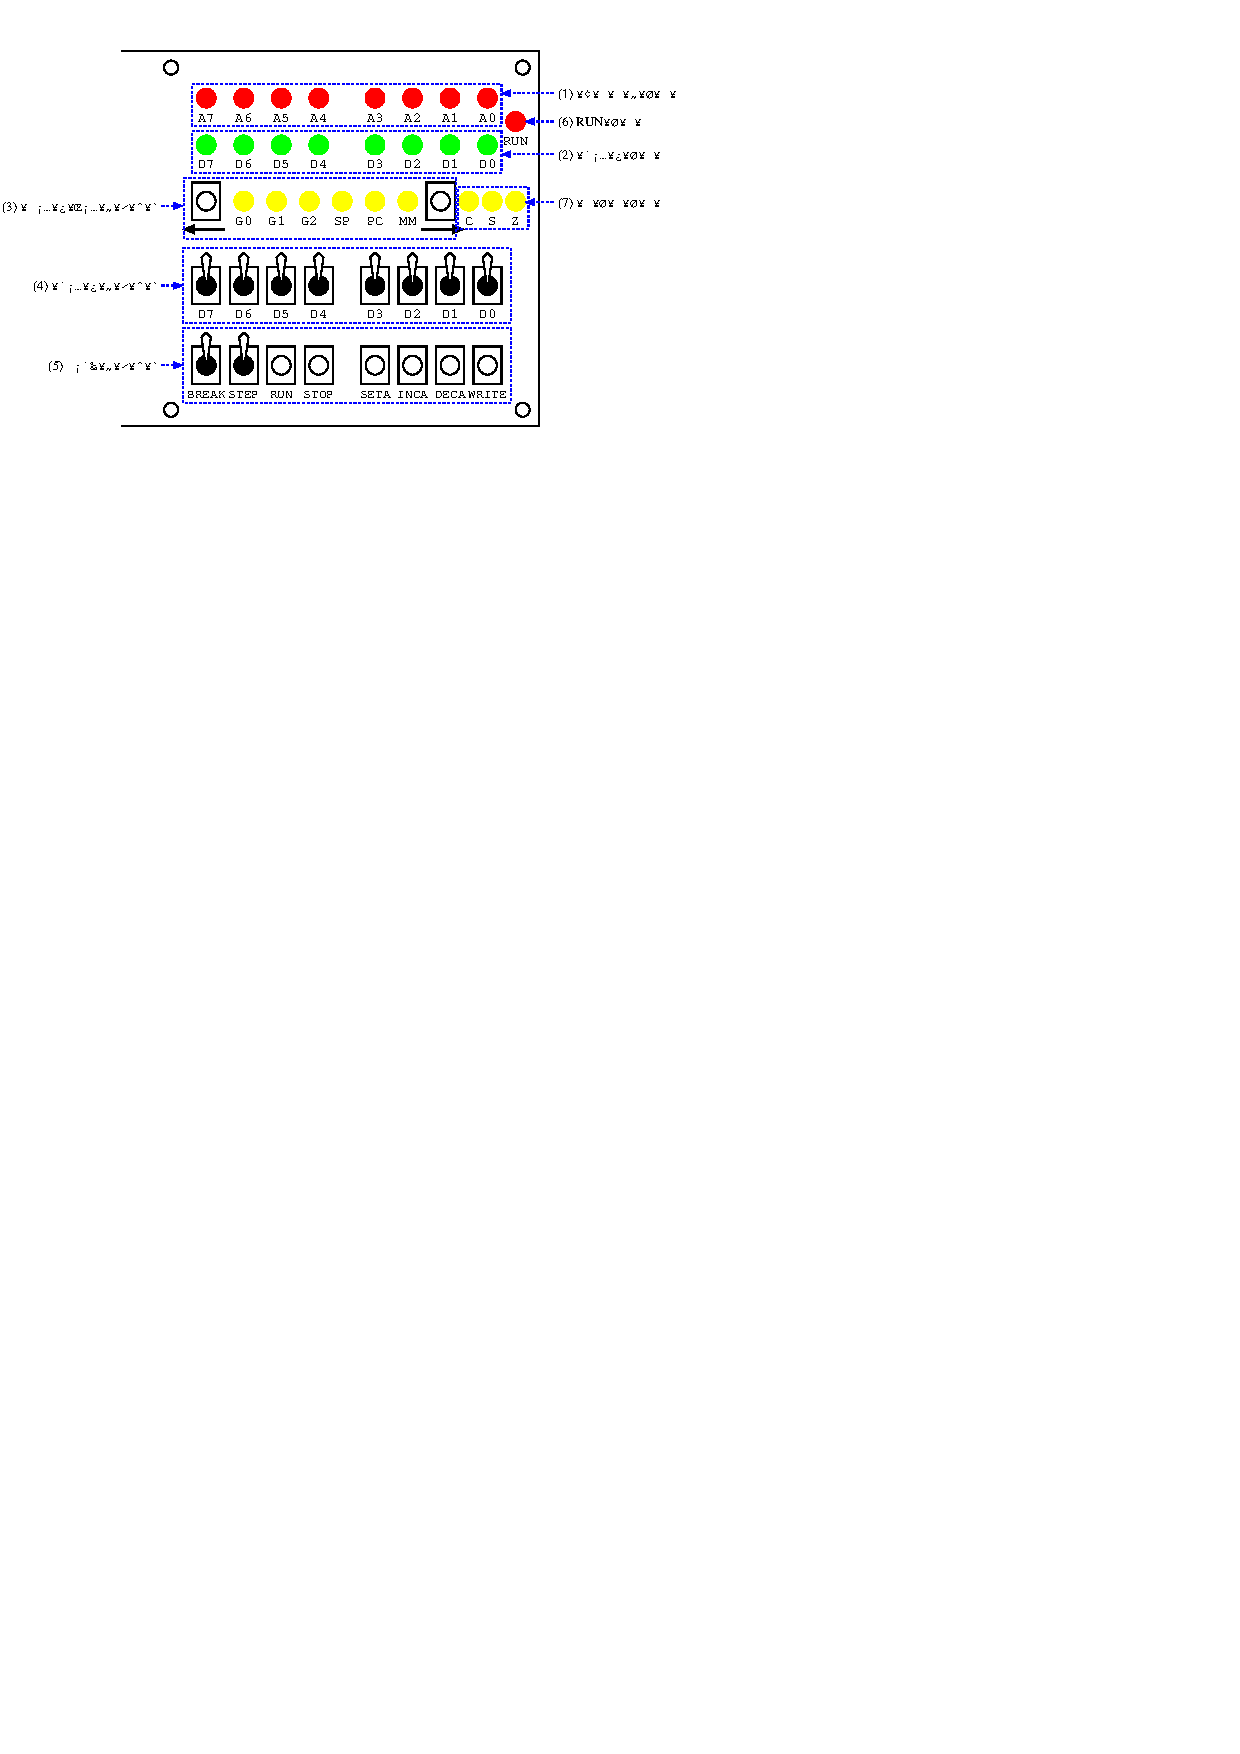
\includegraphics[scale=1.0]{../chap4/console.pdf}}
  \vfill
  \begin{itemize}
    \item ビデオ(各部の名称,後半)
  \end{itemize}
  \vfill
\end{frame}

%==============================================================================
\begin{frame}
  \frametitle{TeC内部の記憶装置}
  \vfill
  \centerline{\includegraphics[scale=0.7]{../chap4/naibu.pdf}}
  \vfill
  \begin{itemize}
    \item ビデオ(TeC内部の記憶装置)
  \end{itemize}
  \vfill
\end{frame}

%==============================================================================
\begin{frame}
  \frametitle{記憶装置の内容を表示/書込み}
  \begin{itemize}
    \item ビデオ(表示から書込みまで)
    \item フラグ
    \item レジスタ
    \item 主記憶(メモリ)
  \end{itemize}
  \vfill
  \vfill
  \vfill
\end{frame}

%==============================================================================
\begin{frame}
  \frametitle{プログラムの実行}
  \begin{itemize}
    \item 主記憶にプログラムを書き込む.
    \item PC(プログラムカウンタ)
    \item STEP,BREAKスイッチ
    \item RESET,RUNスイッチ
  \end{itemize}
  \vfill
  \vfill
  \vfill
\end{frame}

%==============================================================================
\begin{frame}
  \frametitle{練習問題1}
  次のプログラムを実行しなさい.(プログラムは16進数で書く)
  \begin{enumerate}
    \item[1.] 主記憶にプログラムを書き込む.\\
      \begin{tabular}{c c l}
        番地 & データ & コメント \\
        00   & 13     &          \\
        01   & 0A     &          \\
        02   & 17     &          \\
        03   & 0F     &          \\
        04   & 1B     &          \\
        05   & A0     &          \\
        06   & 1F     &          \\
        07   & F0     &          \\
        08   & FF     &          \\
      \end{tabular}
    \item[2.] 00 番地から実行する.
    \item[3.] 実行後の各レジスタの値は?
    \item[4.] STEP実行を用いて各命令の意味を推定する.→コメントに書く
  \end{enumerate}
\end{frame}

%==============================================================================
\begin{frame}
  \frametitle{練習問題2(前半)}
  どのような命令が含まれているか推定しなさい.
  \begin{enumerate}
    \item[1.] プログラム1\\
      \begin{tabular}{c c l}
        番地 & データ & コメント \\
        00   & 13     &          \\
        01   & 01     &          \\
        02   & 33     &          \\
        03   & 01     &          \\
        04   & FF     &          \\
      \end{tabular}
    \item[2.] プログラム2\\
      \begin{tabular}{c c l}
        番地 & データ & コメント \\
        00   & 13     &          \\
        01   & 01     &          \\
        02   & 33     &          \\
        03   & 01     &          \\
        04   & A0     &          \\
        05   & 02     &          \\
      \end{tabular}
  \end{enumerate}
\end{frame}

%==============================================================================
\begin{frame}
  \frametitle{練習問題2(後半)}
  \begin{enumerate}
    \item[3.] プログラム3\\
      \begin{tabular}{c c l}
        番地 & データ & コメント \\
        00   & 13     &          \\
        01   & 01     &          \\
        02   & 20     &  メモリの$10_{16}$番地に何か起こる \\
        03   & 10     &          \\
        04   & FF     &          \\
      \end{tabular}
  \end{enumerate}
  \vfill
\end{frame}

%==============================================================================
\begin{frame}
  \frametitle{期末試験について}
  \begin{enumerate}
  \item[1.] 試験範囲
    \begin{itemize}
    \item 中間試験の範囲に加えて第4章
    \item 第4章の内容は,操作方法,プログラムの実行と実行結果の確認
    \end{itemize}
  \item[2.] 持ち込み物品\\
    TeC本体,ケース,電源ケーブル
  \item[3.] 試験の準備 \\
    \begin{itemize}
    \item 中間試験の範囲を良く復習する.
    \item 教科書の第4章を良く読む.
    \item ビデオ(教科書21ページのQRコード)を良く見る.
    \item 実際にTeCで試してみる.
    \end{itemize}
  \item[4.] 参考(過去問) \\
    練習問題として活用してください.\\
    \url{https://github.com/tctsigemura/Exam/tree/master/FCE}
  \end{enumerate}
  \vfill
\end{frame}

%==============================================================================
%\begin{frame}
%  \frametitle{}
%\end{frame}

\end{document}
